\documentclass[journal=jcisd8,manuscript=article]{achemso}
\usepackage{graphicx}
\usepackage{xr-hyper}
\usepackage{hyperref}
\usepackage{subcaption}
\usepackage[table]{xcolor}
\usepackage{verbatim}
\usepackage[subrefformat=parens]{subcaption}
\usepackage[version=3]{mhchem} % Formula subscripts using \ce{}

\author{Andrew McNutt}
\author{Paul Francoeur}
\affiliation[University of Pittsburgh]
{Department of Computational and Systems Biology, University of Pittsburgh, Pittsburgh, PA}
\author{Rishal Aggarwal}
\affiliation[International Institute of Information Technology Hyderabad]
{Center for Computational Natural Sciences and Bioinformatics, International Institute of Information Technology, Hyderabad 500 032, India}
\author{Tomohide Masuda}
\affiliation[University of Pittsburgh]
{Department of Computational and Systems Biology, University of Pittsburgh, Pittsburgh, PA}
\author{Rocco Meli}
\affiliation[Oxford]{Oxford}
\author{Matthew Ragoza}
\author{Jocelyn Sunseri}
\author{David Ryan Koes}
\email{dkoes@pitt.edu}
\affiliation[University of Pittsburgh]
{Department of Computational and Systems Biology, University of Pittsburgh, Pittsburgh, PA}

\title{Supporting Information:\\GNINA 1.0: Molecular docking with deep learning}
\renewcommand{\thetable}{S\arabic{table}}  
\renewcommand{\thefigure}{S\arabic{figure}}
\begin{document}
\begin{figure}
    \centering
    \begin{subfigure}[b]{0.32\textwidth}
        \centering
        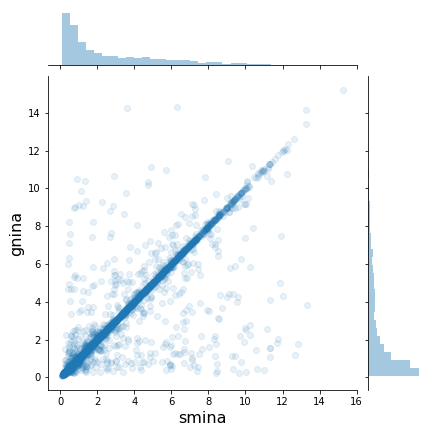
\includegraphics[width=\textwidth]{figures/firstpose.png}
        \caption{First Pose}
        \label{fig:SminaCompareOne}
    \end{subfigure}
    \begin{subfigure}[b]{0.32\textwidth}
        \centering
        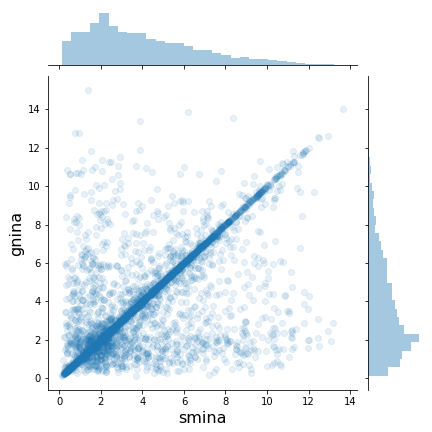
\includegraphics[width=\textwidth]{figures/secondpose.png}
        \caption{Second Pose}
        \label{fig:SminaCompareTwo}
    \end{subfigure}
    \begin{subfigure}[b]{0.32\textwidth}
        \centering
        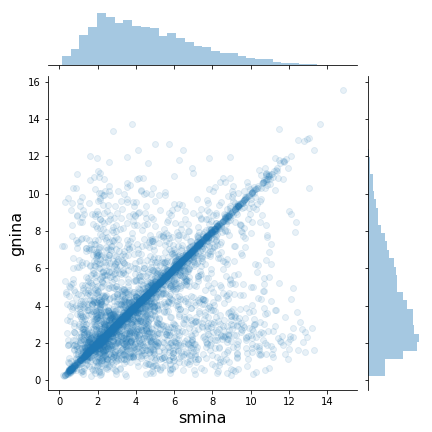
\includegraphics[width=\textwidth]{figures/thirdpose.png}
        \caption{Third Pose}
        \label{fig:SminaComparePose}
    \end{subfigure}
    \caption{Comparison of the RMSD(\AA) of the top 3 poses output by \textsc{Gnina} with no CNN in the docking pipeline and \textsc{Smina}. Both docking software were run with the same arguments.}
    \label{fig:SminaComparePose}
\end{figure}
\begin{figure}
    \centering
    \begin{subfigure}[b]{0.48\textwidth}
        \centering
        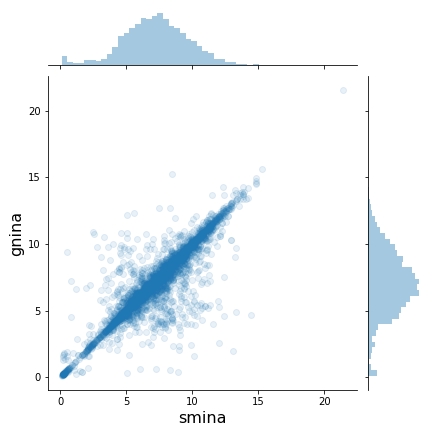
\includegraphics[width=\textwidth]{figures/minpose.png}
        \caption{Minimum RMSD(\AA) Pose}
        \label{fig:SminaCompareMin}
    \end{subfigure}
    \begin{subfigure}[b]{0.48\textwidth}
        \centering
        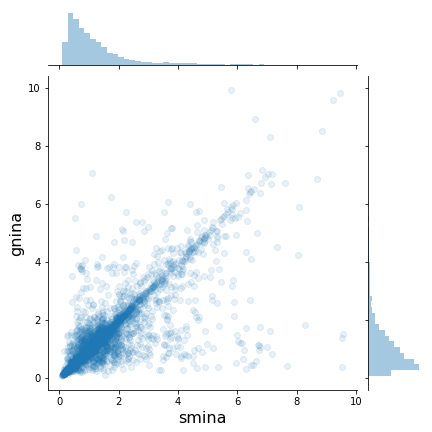
\includegraphics[width=\textwidth]{figures/maxpose.png}
        \caption{Maximum RMSD(\AA) Pose}
        \label{fig:SminaCompareMax}
    \end{subfigure}
    \caption{Comparison of the minimum and maximum RMSD(\AA) poses output by Gnina with no CNN in the docking pipeline and Smina. Both docking software were run with the same arguments.}
    \label{fig:SminaCompareExtrema}
\end{figure}

\begin{table}[]
    \centering
    \begin{tabular}{|c|c|c|c|c|c|}
       \hline\begin{tabular}{{@{}c@{}}}Iteration\\\#\end{tabular}&\begin{tabular}{{@{}c@{}}}Model\\ Selected\end{tabular}&\begin{tabular}{{@{}c@{}}}Redocking\\ Performance\end{tabular}&\begin{tabular}{{@{}c@{}}}Redocking\\Ranking\end{tabular}&\begin{tabular}{{@{}c@{}}} Crossdocking\\Performance\end{tabular}&\begin{tabular}{{@{}c@{}}}Crossdocking\\Ranking\end{tabular}\\ \hline
        0 & Crossdock Dense 4 & 37.8 & 5 & 67.7 & 1 \\ \hline
        1 & General Default2018 3 & 70.4 & 6 & 39.8 & 2 \\ \hline
        2 & Crossdock Dense 3 & 71.2 & 7 & 40.4 & 2 \\ \hline
        3 & Crossdock Default2018 0 & 71.7 & 7 & 40.6 & 2 \\ \hline
        4 & Redock Default2018 2 & 72.2 & 1 & 40.1 & ? \\ \hline
    \end{tabular}
    \caption{Optimal Model Ensemble Selection. Performance given by percent of systems with RMSD less than $2\,\mathrm{\AA}$ from the top pose to the known binding pose.}
    \label{tab:OptimalModelSelection}
\end{table}

\begin{figure}    
        \begin{subfigure}[b]{0.48\textwidth}    
		\centering
		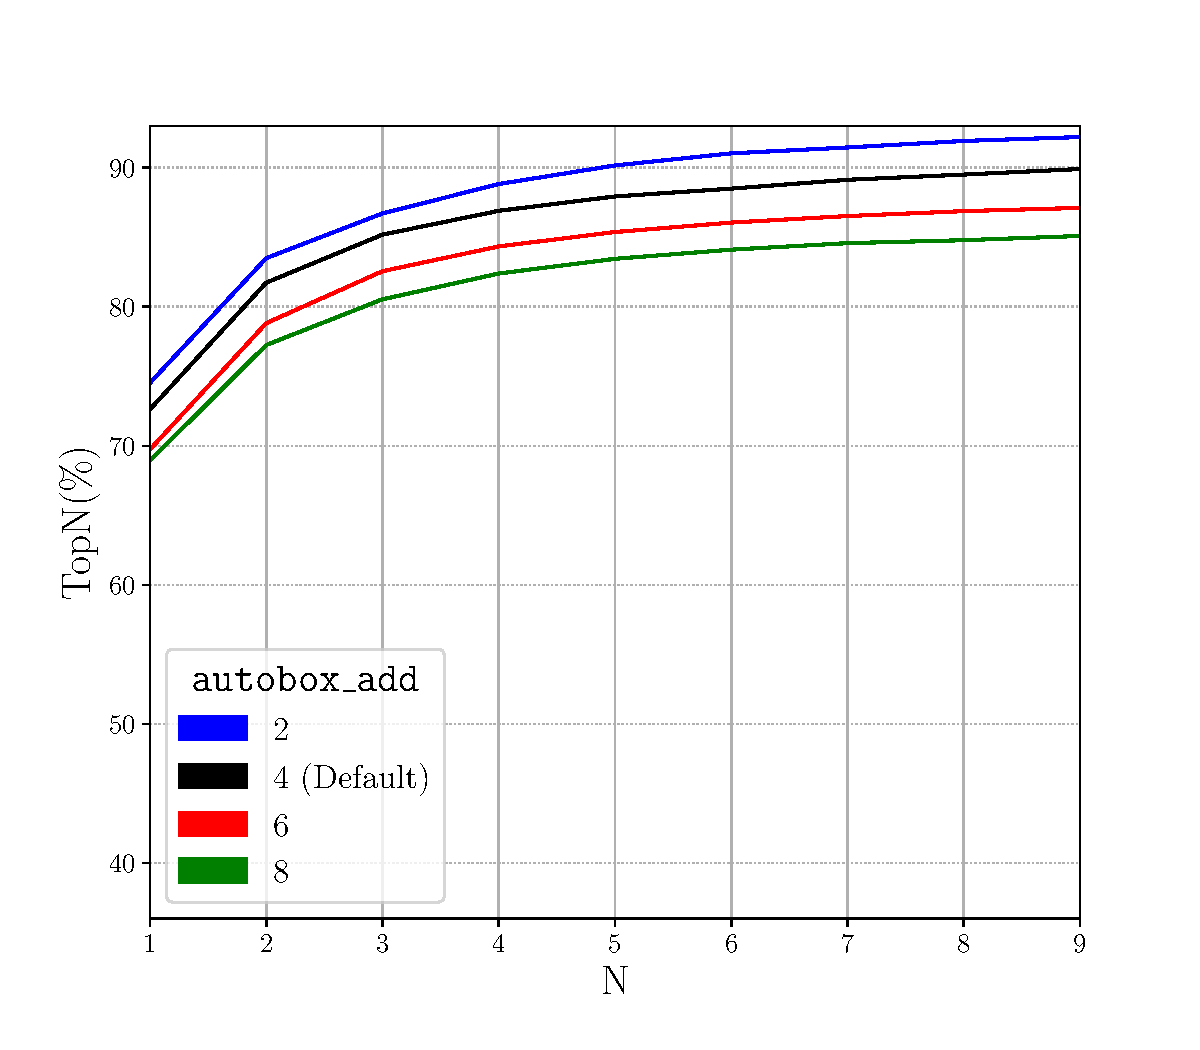
\includegraphics[width=\textwidth]{figures/redocking/sweep_autobox_add_line.pdf}
		\caption{Redocking}
		\label{fig:AutoboxAddRedock}
        \end{subfigure}    
        \begin{subfigure}[b]{0.48\textwidth}    
		\centering
		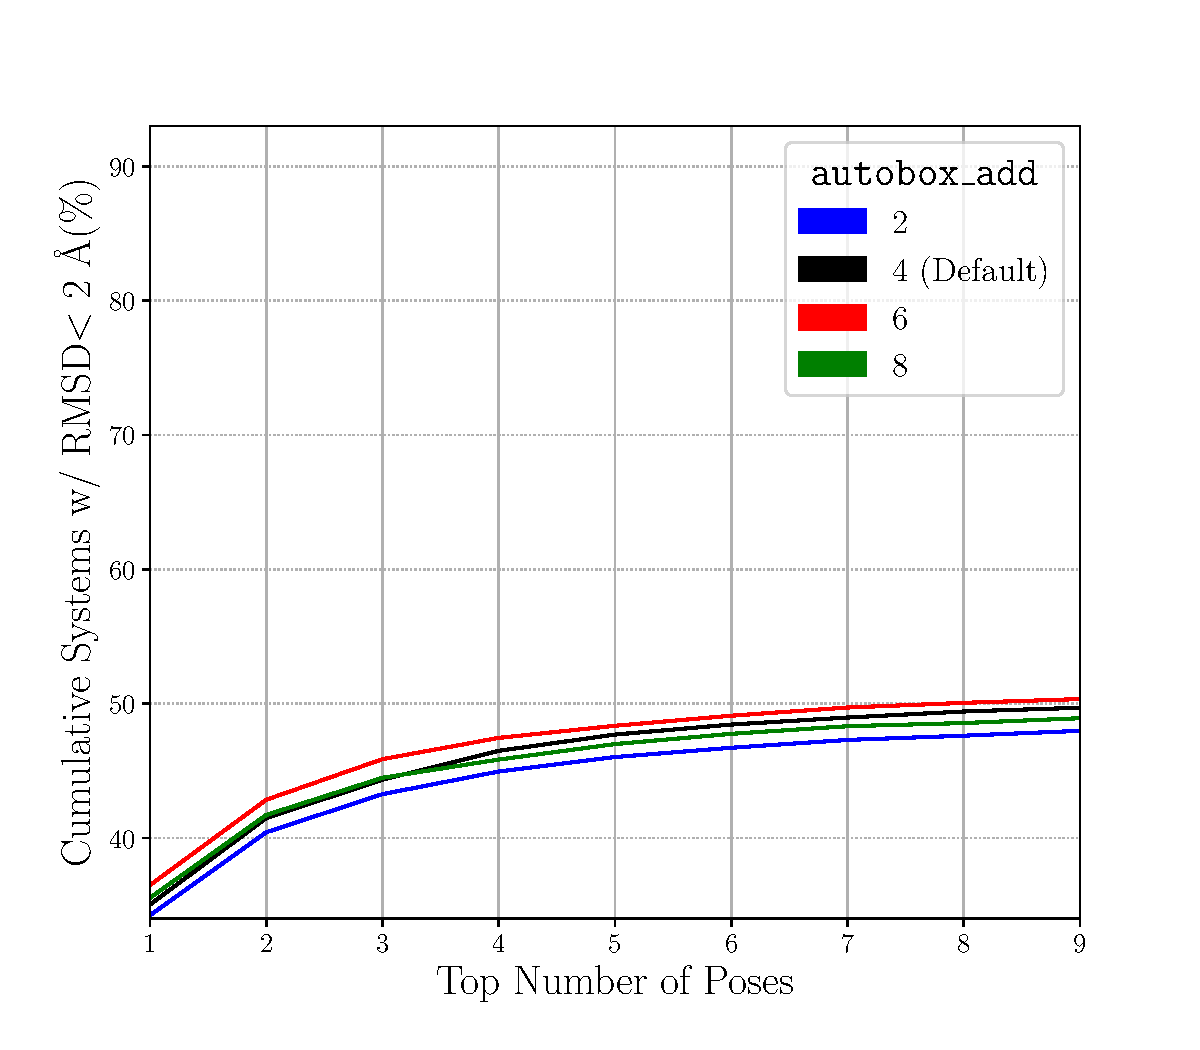
\includegraphics[width=\textwidth]{figures/crossdocking/sweep_autobox_add_line.pdf}
		\caption{Crossdocking}
		\label{fig:AutoboxAddCrossdock}
        \end{subfigure}    
	\caption{Evaluating the effect on docking performance when the value of Autobox Add is changed while using the Default Ensemble for Rescoring on both the redocking and crossdocking datasets.}
	\label{fig:AutoboxAdd}
\end{figure}  

\begin{figure}    
        \begin{subfigure}[b]{0.48\textwidth}    
		\centering
		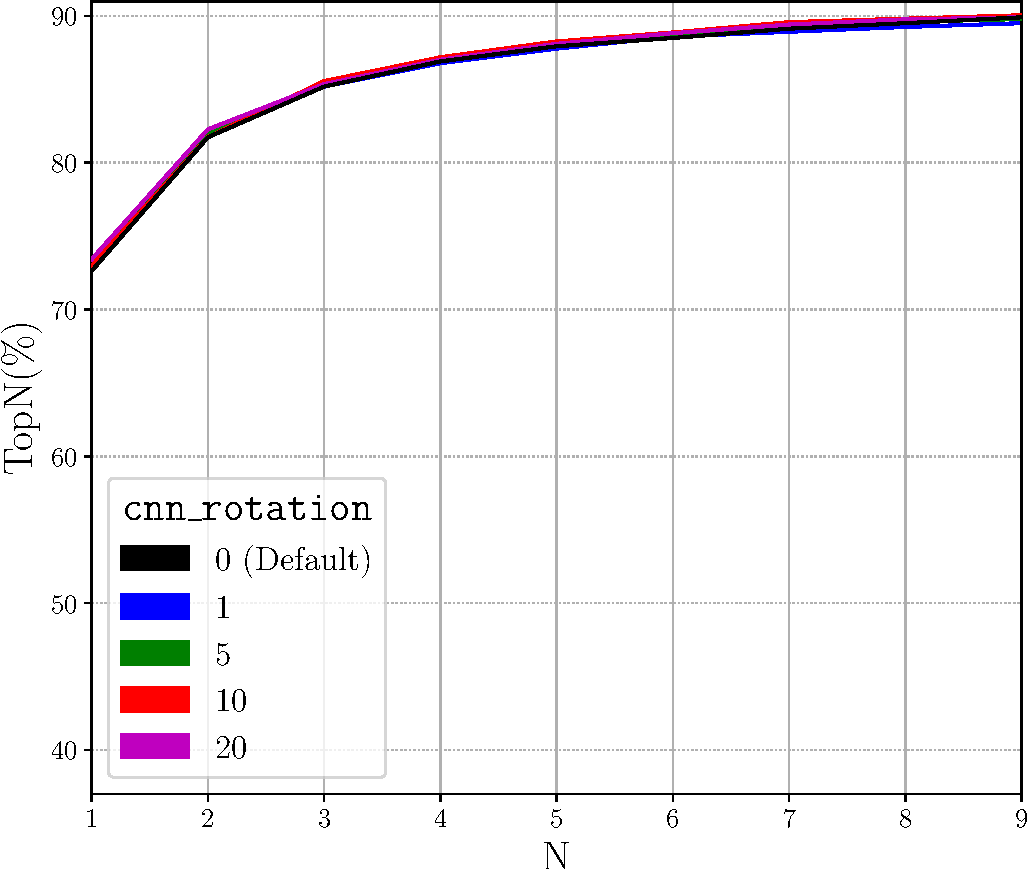
\includegraphics[width=\textwidth]{figures/redocking/sweep_cnnrot_line.pdf}
		\caption{Redocking}
		\label{fig:CNNRotRedock}
        \end{subfigure}    
        \begin{subfigure}[b]{0.48\textwidth}    
		\centering
		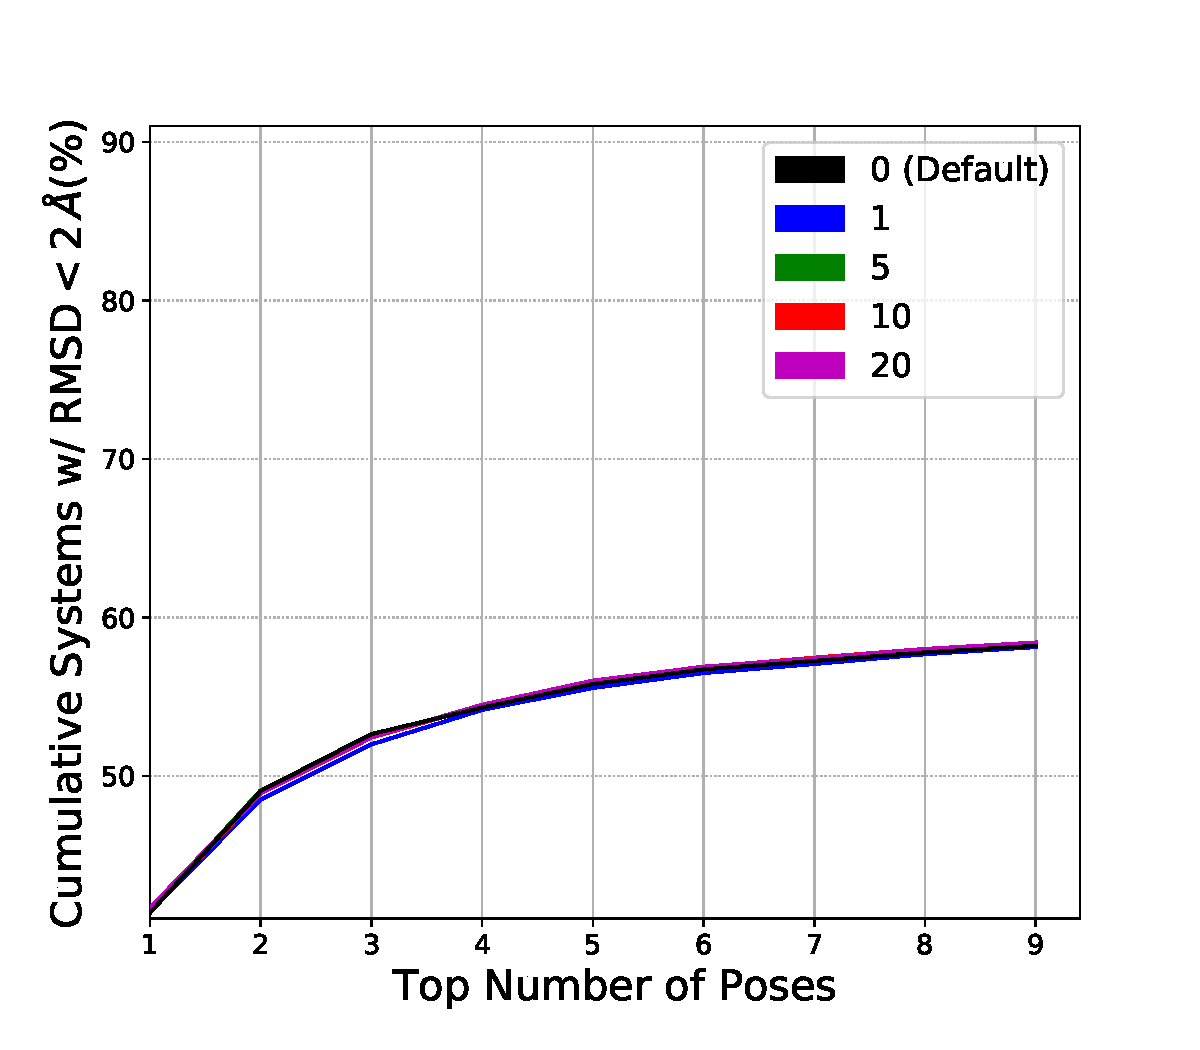
\includegraphics[width=\textwidth]{figures/crossdocking/sweep_cnnrot_line.pdf}
		\caption{Crossdocking}
		\label{fig:CNNRotCrossdock}
        \end{subfigure}    
	\caption{Evaluating the effect on docking performance when the value of CNN rotations is changed while using the Default Ensemble for Rescoring on both the redocking and crossdocking datasets. When CNN rotations is set to 0 the CNN sees a randomly rotated grid of the ligand conformation.}
	\label{fig:CNNRot}
\end{figure}  
\begin{figure}    
        \begin{subfigure}[b]{0.48\textwidth}    
		\centering
		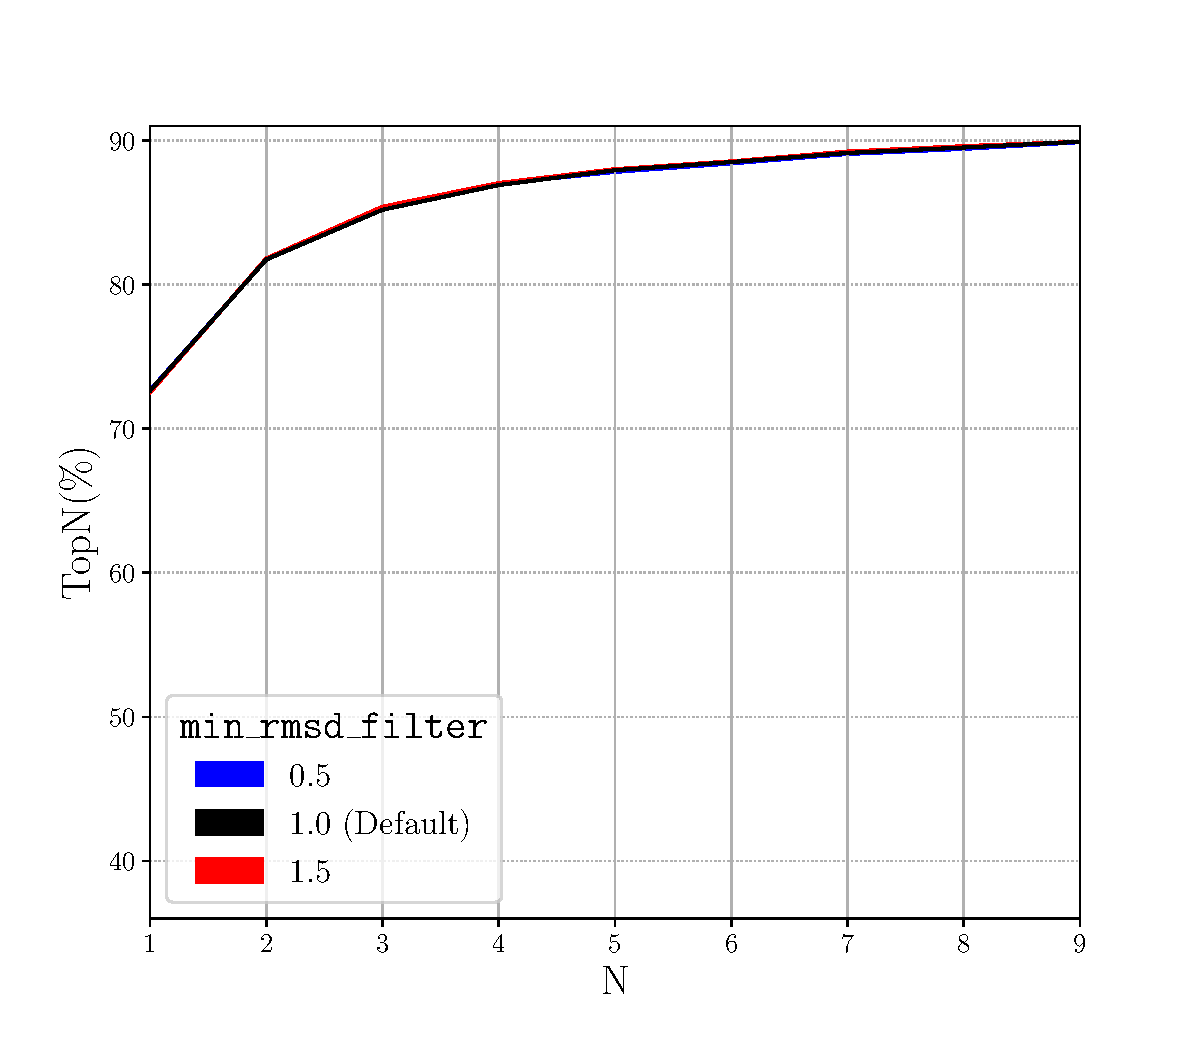
\includegraphics[width=\textwidth]{figures/redocking/sweep_rmsdf_line.pdf}
		\caption{Redocking}
		\label{fig:RMSDFilterRedock}
        \end{subfigure}    
        \begin{subfigure}[b]{0.48\textwidth}    
		\centering
		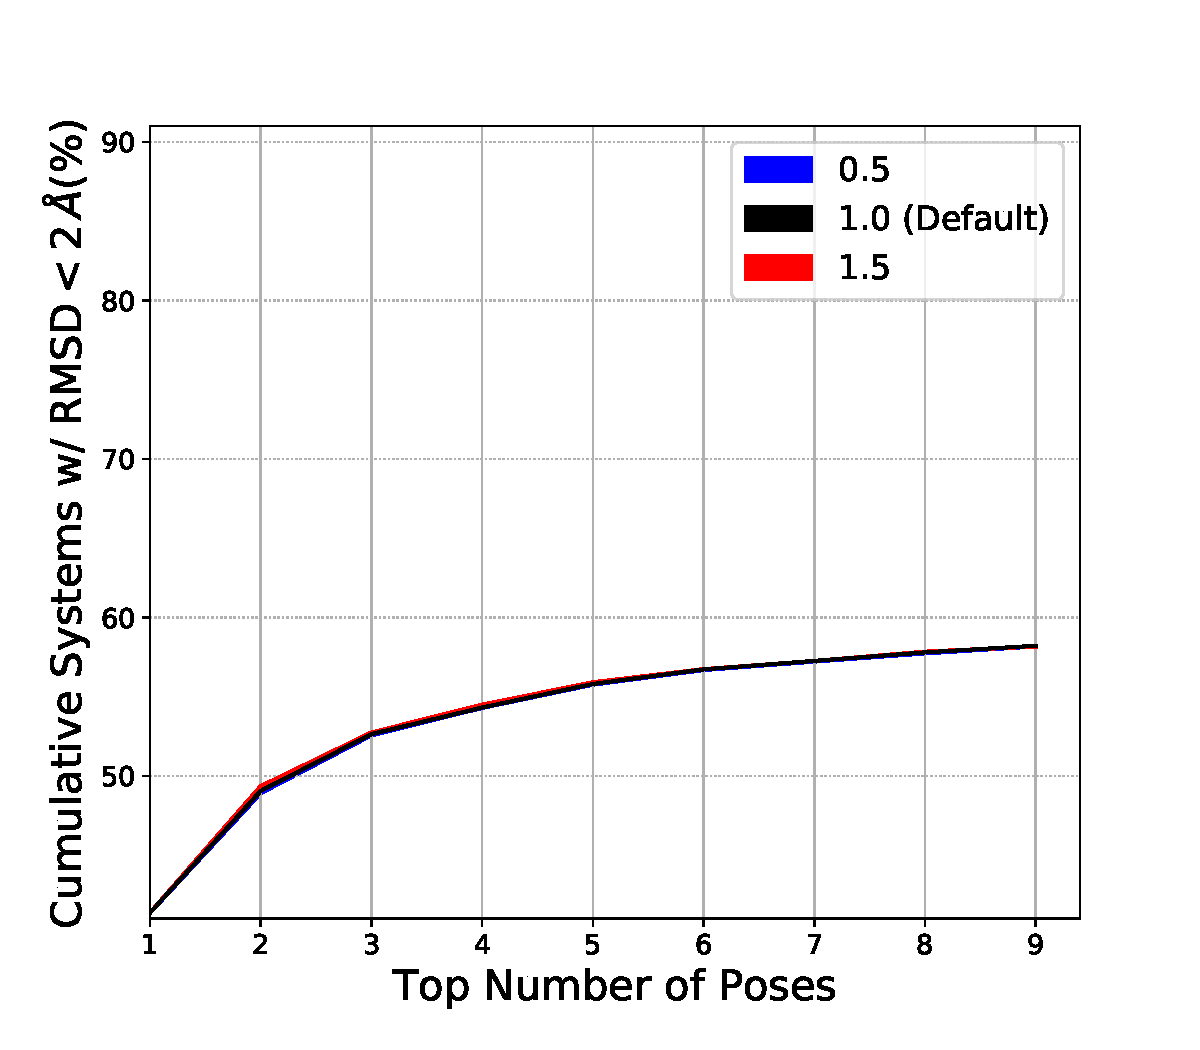
\includegraphics[width=\textwidth]{figures/crossdocking/sweep_rmsdf_line.pdf}
		\caption{Crossdocking}
		\label{fig:RMSDFilterCrossdock}
        \end{subfigure}    
	\caption{Evaluating the effect on docking performance when the value of minimum RMSD filter is changed while using the Default Ensemble for Rescoring on both the redocking and crossdocking datasets.}
	\label{fig:RMSDFilter}
\end{figure}  
\end{document}
